\section{Modification of Streaktubes}

\subsection{Implementation of Fine Grid Velocities}
With all three of the previous implementations we found the remaining existence of fine grid interfacial perturbations. While the fine grid height function method does provide a more rigorous representation of curvature, it does not reduce or remove these perturbations which are nonphysical and lead to the eventual failure of the simulation. To actively reduce the influence of these perturbations a fine grid velocity is implemented based on the work of Herrmann~\cite{Herrmann2013}. This method utilizes a spring-damper analogy to approximate interface motion and is derived  originally from the Taylor analogy breakup model (TAB) of O'Rouke and Amsden~\cite{TAB}. The update equation proposed by Herrmann  is 
\begin{equation}
\frac{\partial \bm{u}_{\text{fg}}}{\partial t} +
(\bar{\bm{u}}+\bm{u}_{\text{fg}}) \cdot \nabla \bm{u}_{\text{fg}} = \\
c_{\sigma}\frac{\sigma}{\rho}\bar{\kappa}(\kappa_{\text{fg}}-\bar{\kappa})- 
c_{\mu}\frac{\mu}{\rho L^2}\bm{u}_{\text{fg}}\nonumber
\label{eqn:HermEq}
\end{equation}

\noindent where, $\bar{\bm{u}}$ is the resolved velocity,
$\bm{u}_{\text{fg}}$ is the fine grid velocity,
$\sigma$ is the surface tension coefficient,
$\rho$ is density, 
$\bar{\kappa}$ is the resolved curvature,
$\kappa_{\text{fg}}$ is the fine grid curvature,
$\mu$ is the dynamic viscosity,
$L$ is a modeling length scale and
$C_\sigma$ and
$C_\mu$ are surface tension and viscous scaling coefficients, respectively~\cite{Herrmann2013}. 
The left side of the equation includes a velocity time rate of change as well as a convective term, while the right side includes the surface tension term which acts as a spring force and the viscous term which is analogous to a damping force. By this analogy, system behavior can be moderated by scaling the value on the surface tension or viscous coefficients. One important feature of this method is that it incorporates a difference of coarse grid curvature ($\bar{\kappa}$) and fine grid curvature ($\kappa_{\text{fg}}$). While there are several ways to approximate this difference, assume the coarse grid curvature is computed using a standard height function method and the fine grid curvature is computed using a second order height function approximation. Other options will be detailed in later sections.
The generalized update algorithm can be summarized as 
\begin{enumerate}
	\item Solve for coarse grid curvature, $\kappa$
	\item Solve for fine grid curvature , $\kappa_{\text{fg}}$
	\item Interpolate coarse grid velocity components to subcell center
	\item Compute the gradient of velocity
	\item Compute normal vector 
	\item Compute viscous term 
	\item Compute density term
	\item Determine accompanying fine grid velocity terms (for $\bm{x}$ direction, $\bm{v}$ \& $\bm{w}$ terms are needed) 
	\item Update fine grid velocity value at cell face
	\item Iterate through time
\end{enumerate}

 The update equation using equation~\ref{eqn:HermEq}, simplified to one-dimension can be written as 

\begin{equation}
 \bm{u_{fg,update}}= 
-(\bar{\bm{u}}+\bm{u}_{\text{fg}}) \cdot \nabla \bm{u}_{\text{fg}} 
-c_{\sigma}\frac{\sigma}{\rho}\bar{\kappa}(\kappa_{\text{fg}}-\bar{\kappa})- 
c_{\mu}\frac{\mu}{\rho L^2}\bm{u}_{\text{fg}}\nonumber
\label{eqn:update}
\end{equation}
which discretizes as 
\begin{multline}
 \bm{u_{\text{fg,update}}}=\\
 - ( \bm{u_{\text{cg}}}(x) + \bm{u_{\text{fg}}}(\text{s,i,j,k}) ) \cdot \nabla \bm{u_{\text{fg,x}}} \\
 - ( \bm{u_{\text{cg}}}(y) + \bm{v_{\text{fg}}}     ) \cdot \nabla \bm{u_{\text{fg,y}}} \\
 - ( \bm{u_{\text{cg}}}(z) + \bm{w_{\text{fg}}}    ) \cdot \nabla \bm{u_{\text{fg,z}}} \\
 - C_{\sigma}\frac{\sigma}{\rho}\kappa(\kappa_{\text{fg}}-\kappa)\bm{n_{\text{x}}} \\
 - C_{\mu} \frac{\mu \bm{u_{\text{fg}}}}{\rho L^2}  \bm{u_{\text{fg}}}(\text{s,i,j,k})
\end{multline}


%RHS_U(s,i,j,k) = &
%- ( VelU(1) + Uf(s,i,j,k) ) * gradUfx &
%- ( VelU(2) + Vfhere      ) * gradUfy &
%- ( VelU(3) + Wfhere      ) * gradUfz &
%- C_sig*sigma/rhoUf*delta*(curvUf-CurvUc)*normUf(1) &
%- C_mu *muUf/rhoUf*L**2*Uf(s,i,j,k)
\noindent and the gradient is discretized using a central finite difference as  

\begin{minipage}{0.25\textwidth}
	\begin{equation*}
	\nabla \bm{u}_{\text{fg,x}}  \rightarrow 
	\end{equation*}\\
\end{minipage}
\begin{minipage}{0.6\textwidth}
	\begin{equation}		
			\frac{\bm{u_{\text{fg}  }(\text{s$^+$,i$^+$,j,k}) - \bm{u_{\text{fg}  }(\text{s$^-$,i$^-$,j,k})} }}  {  \Delta x_{\text{fg}  }}.
	\end{equation}\\
\end{minipage}

\begin{figure}[htbp]
	\centering
	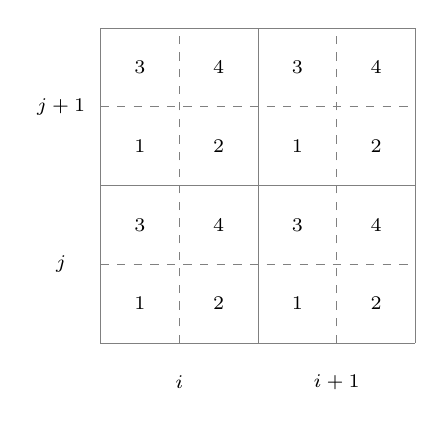
\begin{tikzpicture}[scale=2.0]
	% Mesh
	\draw [step=1.0, help lines] (0 , 0) grid (2,2);
	\draw [dashed,step=0.5, help lines] (0 ,0) grid (2,2);   
	% subcell identifiers
	\node at (0.25,0.25) {\scriptsize $1$};
	\node at (1.25,0.25) {\scriptsize $1$};
	\node at (0.25,1.25) {\scriptsize $1$};
	\node at (1.25,1.25) {\scriptsize $1$};
	
	\node at (0.75,0.25) {\scriptsize $2$};
	\node at (1.75,0.25) {\scriptsize $2$};
	\node at (0.75,1.25) {\scriptsize $2$};
	\node at (1.75,1.25) {\scriptsize $2$};
	
	\node at (0.25,0.75) {\scriptsize $3$};
	\node at (1.25,0.75) {\scriptsize $3$};
	\node at (0.25,1.75) {\scriptsize $3$};
	\node at (1.25,1.75) {\scriptsize $3$};
	
	\node at (0.75,0.75) {\scriptsize $4$};
	\node at (1.75,0.75) {\scriptsize $4$};
	\node at (0.75,1.75) {\scriptsize $4$};
	\node at (1.75,1.75) {\scriptsize $4$};
	
	% Coarse cell id"s
	\node at (0.5,-0.25) {\scriptsize $i$};
	\node at (1.5,-0.25) {\scriptsize $i+1$};
	\node at (-0.25,0.5) {\scriptsize $j$};
	\node at (-0.25,1.5) {\scriptsize $j+1$};
	
	\end{tikzpicture}
	\caption{Fine grid orientation}
	\label{fig:fgOrient}
\end{figure}
\noindent Density and viscous terms are linear averages of the respective phase components, and $\bm{u}_{\text{cg}}$ are interpolated coarse grid velocity components from each respective direction. Note that the $s$ index refers to the fine grid cell and the operator $\text{s$^+$}$ refers to the direction of the adjoining subcell. Illustration of subcell placement can be seen in Figure~\ref{fig:fgOrient}. Because movement within the fine grid can become tedious, NGA incorporates lookup tables which help to minimize confusion. These lookup tables take advantage of the repetitive sequencing of subcell identifiers to ensure accurate referencing of neighboring cells and subcells. \hl{go deeper} 


\subsection*{Correction Incorporation} 
Away from the phase interface, NGA uses high-order finite difference operators that conservatively transport mass, momentum, and any other scalars~\cite{NGA2}.  Near the phase interface however, the finite difference operators are inappropriate due to the discontinuous interface region.  To accurately and conservatively transport near the interface, an unsplit geometric semi-Lagrangian flux method is used~\cite{Owkes2017,Owkes2014}. This method relies on signed streaktubes, which contain the region of the domain that moves through a computational cell face during the timestep~\cite{Owkes2017}.  The streaktube is represented with a collection of tetrahedra as shown in Figures~\ref{fig:streak} \&~\ref{fig:simp} and computational geometry is used to compute the flux of liquid, mass, momentum, and any scalars~\cite{Owkes2017}. A correction is incorporated which forces a solenoidal condition for the cell. Adding the fine-grid velocity correction is done by modifying the additional flux due to the fine-grid velocities. For the finite difference scheme this entails adding the fine-grid velocities associated with a cell face onto the convection velocity at that face. Including the fine-grid velocity requires modifying the streaktubes and in this work two additional tetrahedra are added to each subface such that the volume of the additional tetrahedra is equal to $V_\text{tets}=\Delta t \mathcal{A}_\text{face} \bm{u}_\text{fg}\cdot\bm{n}$. This addition provides an explicit numerical representation of the fine grid velocity correction and maintains conservation laws. 

 \begin{figure}[htbp]
	\centering
	\begin{minipage}{.5\textwidth}
		\centering
		\includegraphics[width=1.0\linewidth]{figs/streaktube.png}
		\caption{fix figure}
		\label{fig:streak}
	\end{minipage}%
	\begin{minipage}{0.5\textwidth}
		\centering
		\includegraphics[width=1.0\linewidth]{figs/simplicies}
		\caption{fix figure}
		\label{fig:simp}
	\end{minipage}
\end{figure}

\subsubsection{Streaktube Mathematical Formulation}
Streaktube development relies on conservation laws applied to a fixed control volume. The following derivation presents advection of a scalar partial differential equation (PDE) into a scalar quantity as it progresses with time due to geometric flux. While the interested reader can be directed to~\ref{1,2,3,4,5,6}  for similar derivations of equation~\ref{eqn:finalStreak}, this derivation is valuable in that it shows exact relations between equation~\ref{eqn:alpha} for a liquid volume fraction ($\alpha$), and equation~\ref{eqn:adv} for a general advected function, $f(x,t)$~\ref{Owkes2017}. This derivation shows that fluxes used within NGA to advect a function through time can be calculated by formulating streaktubes at each cell face of a control volume and evaluating that function at the current timestep. More simply, the derivation provides rigorous validation that any conserved scalar quantity that fluxes through a control volume face at a given timestep can be calculated in the previous timestep as a volumetric quantity and represented geometrically as such as displayed by Figure~\ref{fig:streak}.  

\subsubsection{Derivation}
A conserved scalar $f(\bm{x},t)$ evolves in a solenoidal velocity field as 
\begin{equation}
	\frac{\partial f}{\partial t} + \nabla \cdot (\bm{u} f) = 0
	\label{eqn:der1}
\end{equation}
where \bm{x} is the spatial coordinate value, $t$ is time, and \bm{u} is the velocity field which is known~\ref{Owkes2014}. Integrating this equation over a timestep and the area of a computational cell while using Gauss' theorem on the advection term, we find 
\begin{equation}
\int_{CV} (  f(\bm{x}, t^{n+1})  - f(\bm{x}, t^{n})  ) dV  + \int_{t^n}^{t^{n+1}} \oint_{CV} f \bm{u} \cdot \bm{n}_{CV} dS dt = 0.
	\label{eqn:der2}
\end{equation}
The right term is the surface flux through the control volume and is dependent on $f( \bm{x}, t^{n})$, which is not normally a known quantity. However, a discrete representation of $f( \bm{x}, t^{n})$ is typically known and and update equation can be used to determine $f( \bm{x}, t^{n+1})$. So, the flux is reformulated so that it is solely dependent on $f( \bm{x}, t^{n})$. This is achieved by subdividing the surface of the control volume $CS$ into sub-surfaces $\partial{CS_i}$ such that 
\begin{equation}
	CS = \bigcup_{i=1}^{N_S} \partial CS_i \text{  and  } \\
	\partial CS_i \cap \partial CS_j = 0 \text{ for } i \text{ and } j \in \{1,.....,N_S \} \text{ and } i \not = j
		\label{eqn:der3}
\end{equation}
On each sub-surface $\partial CS_i$ we can link the flux volume $\Omega_i(t)$ to the bounding surface $\omega_i(t)$. $\Omega_i(t)$ is just the signed volume which flows through the sub-surface $\partial CS_i$ over a given timestep $\Delta t$.  The sign of the volume is dependent on the orientation into or out of the control volume and is positive if flowing out of, and negative if flowing into, the control volume~\ref{Owkes2017}. 

Integrating Equation~\ref{eqn:der1} over the flux volume $\Omega_i$ and again using Gauss' theorem on the second term we find 
\begin{equation}
	\int_{\Omega_i(t)} \frac{\partial f}{\partial t} dV  + \oint_{\omega_i(t)} f \bm{u} \cdot \bm{n}_{\Omega_i} dS = 0.
	\label{eqn:der4}
\end{equation}
Here, $\bm{n}_{\Omega_i}$ is the outward facing normal to the flux volume $\Omega_i(t)$. The bounding surface $\omega_i$ is partitioned as $\omega_{i,F} = \omega_i \cap \partial CS_i = \partial CS_i$, which is fixed and $\omega_{i,M} = \omega_i \backslash \partial CS_i $ which is a material surface~\ref{Owkes2017}. This is valid by defining part of $\omega_i$ as having zero flux of $f$ and therefore must move with the flow. The other portion of $\omega_i$ is defined such that it coincides with $\partial CS_i$, which is fixed in time. Intergrating Eq.~\ref{eqn:der4} over time and using the previous partition we find that 
\begin{equation}
	\int_{t^n}^{t^{n+1}} \int_{\Omega_i(t)} \frac{\partial f}{\partial t} dV dt + \int_{t^n}^{t^{n+1}} \int_{\omega_{i,M}(t)} f \bm{u} \cdot \bm{n}_{\Omega_i} dS dt + 	\int_{t^n}^{t^{n+1}} \int_{\partial CS_i} f \bm{u} \cdot \bm{n}_{\Omega_i} dS dt = 0.
	\label{eqn:der5}
\end{equation}
Because of its similarity to the flux term in Eq.~\ref{eqn:der2}, the right term of the above equation will provide a bridge between the two equations. The remaining terms can be made more clear using Leibniz's method which states 
\begin{equation}
	\frac{d}{dt} \int_{\Omega_i(t)} f dV = \int_{\Omega_i(t)} \frac{\partial f}{\partial t} dV + \int_{\omega_{i,M}(t)} f \bm{u} \cdot \bm{n}_{\Omega_i} dS.
	\label{eqn:der6}
\end{equation}
With this, we can see that a $\Omega_i(t)$ is a streaktube projected backward in time from the surface $\partial CS_i$ over the timestep $\Delta t$. Integrating Eq.~\ref{eqn:der6} with time results in 
\begin{equation}
	\int_{\Omega_i(t^{n+1})} f (\bm{x} , t^{n+1}) dV - \int_{\Omega_i(t^{n})} f (\bm{x} , t^{n}) dV  = \int_{t^n}^{t^{n+1}}\int_{\Omega_i(t)} \frac{\partial f}{\partial t} dV dt+ \int_{t^n}^{t^{n+1}} \int_{\omega_{i,M}(t)} f \bm{u} \cdot \bm{n}_{\Omega_i} dS dt.
	\label{eqn:der7}
\end{equation}
By definition, $\Omega_i(t^{n+1})$ is zero, making the first term equal to zero. We can adopt the notation that $\Omega_i=\Omega_i(t^{n})$ and call this term the flux volume. Subtracting Eq.~\ref{eqn:der7} from Eq.~\ref{eqn:der5} we find that 
\begin{equation}
	\int_{t^n}^{t^{n+1}}\int_{\partial CS_i}  f \bm{u} \cdot \bm{n}_{\Omega_i} dS dt = \int_{\Omega_i} f (\bm{x} , t^{n}) dV, 
	\label{eqn:der8}
\end{equation}
which gives us a simple relation between the flux through the sub-surface $\partial CS_i$ and the volume integral over $\Omega_i$.

To obtain a useful time advancement equation we would like to combine Eq.~\ref{eqn:der2} and Eq.~\ref{eq,:der8}. However, doing so requires a relation between the normal terms, $\bm{n}_{CV}$ and $\bm{\Omega}$ as these normals are both defined using the same surface. This means that either, the two normals are identical or face opposite directions. We assume a signed notation for portions of the control surface and associate them with the flux volumes similarly. With this relationship we can finally obtain 
 \begin{equation}
	 \int_{CV} (f (\bm{x} , t^{n+1}) - f (\bm{x} , t^{n}) )dV + \sum_{i=1}^{N_S}\int_{\Omega_S} f (\bm{x} , t^{n}) )dV =0
	 \label{eqn:derFinal}
 \end{equation}
where $\Omega_S$ is now the signed streaktube. The final form provides that the change in the scalar $f$  within the control volume $CV$ over the timestep $\Delta t$ must be equal to the volume integral of the signed flux volumes.

\section{Modification of Fine Grid Velocity}
Initial results of the fine grid velocity method coupled with height function calculation of curvature suggested a fundamental problem. While explicit curvature calculation remained consistent with previous methods, the oscillating droplet test case again proved difficult as seen by Figures~\ref{fig:OGfgVelKE}~\&~\ref{fig:OGfgVelCurv}. Close inspection of Eq.~\ref{eqn:HermEq} reveals that the equation is not well-poised when the coarse-grid curvature, $\bar{\kappa}$, is zero as the entire spring force goes to zero even if fine-grid interface perturbations exist.  An alternative is to base the source term on the difference between coarse and fine-grid curvatures and add a delta function that restricts the source term to only be non-zero at the interface.  The approximation of the Dirac delta function is calculated as the absolute difference in liquid volume fractions between cells divided by the mesh size as in equation~\ref{eqn:delta}.
\begin{equation}
\delta = \frac{|\alpha(\text{s,i,j,k}) - \alpha(\text{s,i-sc,j,k}) | }{0.5 \Delta x}
\label{eqn:delta}
\end{equation}
 Additionally, a pressure term is added to ensure fine grid velocity remains divergence free, further enforcing momentum conservation. With these modifications, the proposed equation to create the fine-grid velocity can be written as

\begin{equation}
\frac{\partial \bm{u}_{\text{fg}}}{\partial t} +
(\bar{\bm{u}}+\bm{u}_{\text{fg}}) \cdot \nabla \bm{u}_{\text{fg}} = 
c_{\sigma}\frac{\sigma}{\rho}\delta(\kappa_{\text{fg}}-\bar{\kappa})- 
c_{\mu}\frac{\mu}{\rho L^2}\bm{u}_{\text{fg}} -
\nabla P_{\text{fg}}\nonumber
\label{eqn:MyEq}
\end{equation}
along with the continuity equation
\begin{equation}
\nabla\cdot\bm{u}_\text{fg}=0.
\end{equation}
The modified update algorithm is 
\begin{enumerate}
	\item Solve for coarse grid curvature, $\kappa$
	\item Solve for fine grid curvature , $\kappa_{\text{fg}}$
	\item Interpolate coarse grid velocity components to subcell center
	\item Compute the gradient of velocity
	\item Compute normal vector 
	\item Compute viscous term 
	\item Compute density term
	\item Determine accompanying fine grid velocity terms (for $\bm{x}$ direction, $\bm{v}$ \& $\bm{w}$ terms are needed) 
	\item Calculate delta function using equation~\ref{eqn:delta}
	\item Update fine grid velocity value at cell face
	\item Solve pressure Poisson equation 
	\item Correct velocity value using updated pressure field 
	\item Iterate through time
\end{enumerate}
% \begin{figure}[htbp]
%	\centering
%	\begin{minipage}{.5\textwidth}
%		\centering
%		\includegraphics[width=1.0\linewidth]{figs/curvCalc.png}
%		\caption{fix figure}
%		\label{fig:OGfgVelCurv}
%	\end{minipage}%
%	\begin{minipage}{0.5\textwidth}
%		\centering
%		\includegraphics[width=1.0\linewidth]{figs/KEvT}
%		\caption{fix figure}
%		\label{fig:OGfgVelKE}
%	\end{minipage}
%\end{figure}

Equation~\ref{eqn:MyEq} is representative of the scheme implemented at the time of this publication. As before, the same explicit curvature calculation and oscillating droplet test cases were conducted. Results are shown in Figures~\ref{fig:fgVelCurv}~\&~\ref{fig:fgVelKE} and show considerable improvement from the standard height function method. However, test cases still resulted in nonphysical dynamics when moving to more complex geometries. All test cases examined which include three dimensional geometry resulted in errors which eventually caused simulation failure. 
\begin{figure}[htbp]
	\centering
	\begin{minipage}{.5\textwidth}
		\centering
		\includegraphics[width=1.0\linewidth]{figs/curvCalc.png}
		\caption{fix figure}
		\label{fig:fgVelCurv}
	\end{minipage}%
	\begin{minipage}{0.5\textwidth}
		\centering
		\includegraphics[width=1.0\linewidth]{figs/current_KEplot.png}
		\caption{fix figure}
		\label{fig:fgVelKE}
	\end{minipage}
\end{figure}
Additional efforts were taken to  find an optimal parameterization strategy with little success. Figure~\ref{fig:para} shows a parameterization study where $C_{\sigma}$ and $C_{\mu}$ varied from $1e^-6$ to $1e^6$ and an oscillating droplet test case was ran. While a portion of the runs seem initially successful, tuned parameter values were not found to be consistent across various mesh sizes and no conclusive optimal configuration was found. Because of this, it seemed appropriate to take a deeper look into determining the mechanisms within the method which are the cause of these failures. 
%\begin{figure}
%	\centering
%	\includegraphics[width=1.0\textwidth]{figs/para}
%	\caption{fix figure}
%	\label{fig:para}
%\end{figure}